{
{\sffamily Vi kaster i det følgende et detaljeret blik på
billedbehandlingsmetoderne i programmet. Efter en kort teknisk
introduktion til digitale billeder, vises hvilke datastrukturer og
metoder \emph{OpenCV} stiller til rådighed og hvordan disse bruges til
at udtrække regioner i digitale billeder. Endeligt vil vi undersøge
hvilke problemer vores implementation kan have.
}

\subsection{Digitale billeder}
I afsnit \ref{section_kort_intro} blev der givet en kort introduktion
til den digitale repræsentation af billeder. Vi antog at en pixel kunne
antage værdier i mængden $\{0, 1\}$. I praksis kan pixels godt tage
andre værdier. Vi arbejder med billeder, hvor værdien for hver pixel, er
repræsenteret ved tre 8 bit størrelser, hver især med værdier i mængden
$\{0, 1, 2, \cdots, 254, 255\}$. Sammensætningen af de tre værdier, som
beskrives som kanaler eller farvebånd, kaldes for en RGB-farve, hvor
tallene repræsenteret ved $(R,G,B)$ henholdsvis angiver mængden af rød,
grøn og blå farve i en pixel. Et sådan billede kaldes for et
RGB-billede.  Vi benytter os af 8 bit størrelsen, da dette er
industristandarden\footnote{Reference}. For en uddybende forklaring om
billeders repræsentation, refereres igen til \cite{SIOlsen}.

Hvordan repræsenteres billeder i \emph{OpenCV}? Skriv det her.

\subsection{Vigtige datastrukturer}
Herunder vil vi gennemgår nogle vigtige datastrukturer som vi bruger fra
\emph{OpenCV}.  Alle datastrukturer og metoder fra \emph{OpenCV} er
prefikset med ``cv'' hvilket gør det let at se hvor koden kommer fra.
Der præsenteres i det følgende en notation for datastrukturer.
Notationen er underlagt strukturen vist i (\ref{types_class}).
\begin{multline}
    \textbf{class~} [\textit{name}] = \{ \\
    \shoveleft{\qquad[\textit{type}] : [\textit{varName}]} \\
    \shoveleft{\}}\shoveright{}
    \label{types_class}
\end{multline}
I (\ref{example_class}) ses et eksempel på en struktur kaldet
\textbf{ExampleClass}.
\begin{multline}
    \textbf{class~} \textrm{ExampleClass} = \{ \\
    \shoveleft{\qquad\textbf{int} : \textit{intValue}} \\
    \shoveleft{\qquad\textbf{string} : \textit{stringValue}} \\
    \shoveleft{\qquad\textbf{int[2]} : \textit{arrayValues}} \\
    \shoveleft{\}}\shoveright{}
    \label{example_class}
\end{multline}
Når en type har et suffiks på formen $\textit{type}[i]$, hvor $i$ er et
heltal, betyder det at dette er en liste af længde $i$ af typen
\textit{type}.  Bemærk, at en strukturs navn bliver skrevet med fed
skrift i brødteksten, når der refereres til en sådan. Ligeledes vil en
strukturs navn blive skrevet med fed i pseudokoden hvis der refereres
til den. Vi kan definere en ny struktur \textbf{NewClass} som viser
dette i (\ref{new_class}) herunder.
\begin{multline}
    \textbf{class~} \textrm{NewClass} = \{ \\
    \shoveleft{\qquad\textbf{ExampleClass} : \textit{exampleInstance}} \\
    \shoveleft{\qquad\textbf{string} : \textit{stringValue}} \\
    \shoveleft{\}}\shoveright{}
    \label{new_class}
\end{multline}
Vi vil nu beskrive de vigtigste strukturer som vi bruger, med
ovenstående notation.

\subsubsection{cvScalar}
Strukturen \textbf{cvScalar} fungerer egentlig blot som en almindelig
liste med værdier. En instans af \textbf{cvScalar} kan dog kun indeholde
1, 2, 3 eller 4 værdier. Strukturen vist i (\ref{cvScalar_class}) har fire
værdier.
\begin{multline}
    \textbf{class~} \textrm{cvScalar} = \{ \\
    \shoveleft{\qquad\textbf{double[4]} : \textit{value}} \\
    \shoveleft{\}}\shoveright{}
    \label{cvScalar_class}
\end{multline}
I \emph{OpenCV}, og vores implementation i øvrigt, bruges strukturen
blandt andet til RGB-farver og tærskelværdier.

\subsubsection{cvPoint}
Strukturen \textbf{cvPoint} har til formål at beskrive punkter i det
to-dimensionelle plan. Den er givet i (\ref{cvPoint_class}).
\begin{multline}
    \textbf{class~} \textrm{cvPoint} = \{ \\
    \shoveleft{\qquad\textbf{int} : \textit{x}} \\
    \shoveleft{\qquad\textbf{int} : \textit{y}} \\
    \shoveleft{\}}\shoveright{}
    \label{cvPoint_class}
\end{multline}
Strukturen er simpel, men er en meget central del af implementationen.
Den bruges blandt andet til at angive snit i billedet og fortælle
floodfill hvor vi skal male og skifte farve.

\subsubsection{cvRect}
Denne struktur beskriver et rektangel ved at angive dets øverste venstre
hjørne og dimensioner. Strukturen vises i (\ref{cvRect_class}).
\begin{multline}
    \textbf{class~} \textrm{cvRect} = \{ \\
    \shoveleft{\qquad\textbf{int} : \textit{x}} \\
    \shoveleft{\qquad\textbf{int} : \textit{y}} \\
    \shoveleft{\qquad\textbf{int} : \textit{height}} \\
    \shoveleft{\qquad\textbf{int} : \textit{width}} \\
    \shoveleft{\}}\shoveright{}
    \label{cvRect_class}
\end{multline}
I vores implementation af den naive fremgangsmåde, som nævnt i afsnit
\ref{section_naiv}, er det denne struktur som angiver en regions
afgrænsende rektangel. Vi vil i afsnit \ref{section_vurdering_regioner}
se hvordan strukturen \textbf{cvRect} bruges til at vurdere om regioner
ligger i det gyldne snit. Først skal vi dog lige se på metoderne der
bruges til at trække regionerne ud af billedet.

\subsubsection{Line}
Den sidste struktur vi vil nævne kommer ikke fra \emph{OpenCV}, men er
blevet udviklet med henblik på at repræsentere snit i billeder.
Strukturen \textbf{Line} er reelt bare en linjestykke og har strukturen
vist i (\ref{Line_class}).
\begin{multline}
    \textbf{class~} \textrm{cvRect} = \{ \\
    \shoveleft{\qquad\textbf{cvPoint} : \textit{p1}} \\
    \shoveleft{\qquad\textbf{cvPoint} : \textit{p2}} \\
    \shoveleft{\}}\shoveright{}
    \label{Line_class}
\end{multline}

\subsection{Resultaters struktur\label{resultat_struktur}}
Vi definerer en ny struktur der repræsenterer Pythons \emph{dictionary},
som vi vil forkorte \emph{dict}. I praksis er det en liste som man slår
op i vedbrug af en nøgle. Nøglen kan være hvilken som helst type, men er
gerne en streng eller et heltal. Til hver indgang i listen er der
tilknyttet noget data som også kan være af en vilkårlig type. Man kan
derved have \emph{dicts} inde i en \emph{dict}. En \emph{dict} defineres
som vist i \ref{def_dict}.
\begin{eqnarray}
    \langle[\textit{dictName}]\rangle = \{ [\textit{key}] : [\textit{data}] \}
    \label{def_dict}
\end{eqnarray}
Som et simpelt eksempel kan vi konstruere en \emph{dict}
$\angles{LuckyNumbers}$ som indeholder personers lykketal:
% TeX-Gods, please forgive me :(
\begin{multline}
    \angles{LuckyNumbers} = \{ \qquad \textrm{Tom Cruise} : 4 , \\
    \textrm{Arthur Dent} : 42 \qquad\qquad\\
    \shoveleft{\}}\shoveright{}
    \label{lucky_dict}
\end{multline}
% In honor of the danish Tom Cruise

\begin{multline}
    \angles{CutRegions} = \{ \textit{~RegionId} : \\
    (\textbf{cvScalar~}\textit{color}, \textbf{cvConnectedComp~}\textit{component}) \}\quad
\end{multline}

\begin{eqnarray}
    \angles{RatioRegions} = \{ \textit{~CutNo} : \angles{CutRegions} \}
\end{eqnarray}

\begin{eqnarray}
    \angles{ImageRegions} = \{ \textit{~CutRatio} : \angles{RatioRegions} \}
\end{eqnarray}

\subsection{Centrale metoder}
Dette afsnit vil introducere de centrale metoder fra \emph{OpenCV} som
vi gør brug af.  Når der i brødteksten refereres til metoder, noteres de
med skrivemaskineskrift.

\subsubsection{Kantdetektion og sløring}
Som nævnt i afsnit \ref{udtraek_kanter}, bruger vi kantdetektionsmetoden
Canny. \emph{OpenCV} har implementeret denne metode som
\texttt{cvCanny}. Metoden skal køres på et sort/hvid-billede, så vi
starter med at lave en sort/hvid kopi af det originale billede. Vi skal
også bruge et tomt output-billede hvor kanterne kan tegnes i. Dette skal
ligeledes være et sort/hvid-billede. Resultatet fra \texttt{cvCanny} er
tidligere vist i figurene \ref{canny_kanter} og \ref{sammen_kanter}.

\emph{OpenCV} stiller metoden \texttt{cvSmooth} til rådighed for sløring
af billeder. \texttt{cvSmooth} tager som argumenter det oprindelige
billede, et billede hvori resultatet vises, dimensionerne på
foldningsmatricen der skal bruges og endelig hvilken sløringsmetode der
ønskes brugt. Vi har metoderne vist i afsnit \ref{udtraek_sloering} til
rådighed. Vi bruger simpel sløring på billedet inden kantdetektion, da
vi på denne måde kun betragter kanter som fremstår tydeligt i billedet.
Simpel sløring er hurtigt og effektiv, og bliver derfor også brugt på
billedet inden vi bruger floodfill.

\paragraph{Fremhævning af kanter}
Inverter det kantdetekterede billede, brug det som mask når det
originale kopires over i et sort billede. Derved bliver pixels med en
kant ikke farvet, dvs. de forbliver sorte.

\subsubsection{Floodfill}
\emph{OpenCV} har implementeret floodfill metoden i
\texttt{cvFloodFill}. Metoden introducerer en ny datastruktur, der
beskriver den region som \texttt{cvFloddFill} har fundet. Strukturen er
vist i (\ref{cvConnectedComp_class}).
\begin{multline}
    \textbf{class~} \textrm{cvConnectedComp} = \{ \\
    \shoveleft{\qquad\textbf{double} : \textit{area}} \\
    \shoveleft{\qquad\textbf{float} : \textit{value}} \\
    \shoveleft{\qquad\textbf{cvRect} : \textit{rect}} \\
    \shoveleft{\}}\shoveright{}
    \label{cvConnectedComp_class}
\end{multline}
Strukturen indeholder en regions afgrænsende rektangel og regionens
areal.  På baggrund af disse værdier tages beslutningen om en region er
interessant, og om en interessant region ligger i det gyldne snit,
hvilket vi vil komme nærmere ind på i afsnit
\ref{section_vurdering_regioner}.  I nyere versioner af \emph{OpenCV}
indeholder strukturen den eksakte sekvens af punkter som udgør
komponentens kanter.

\subsection{Udtrækning af regioner}
Informationerne fra et kantdetekteret billede kan hjælpe
\texttt{cvFloodFill} til at trække regioner ud af billedet. Hvis vi har
et snit repræsenteret ved en instans af strukturen \textbf{Line}, kan vi
gemme punkterne hvor en kant krydser snittet. Et eksempel ses i figur
\ref{impUdtraek_kantpunkter}, hvor vi har et horisontalt snit
repræsenteret ved linjestykket $AB$ og punkterne $e_1, \cdots, e_6$ er
der hvor en kant krydser. Vi antager i det følgende, at pixels i
billedet vi undersøger, har RGB-værdier i mængden
$\{(0,0,0),(255,255,255)\}$, hvilket vil sige at billedets pixels enten
er helt sorte eller helt hvide, billedet vi undersøger er binært.

\begin{figure}[!h]
    \centering
    \begin{picture}(240,30)
        \put(0, 10){$A$}
        \put(3, -5){\line(0, 1){10}}

        \put(82, 10){$e_1$}
        \put(85, 0){\circle*{3}}

        \put(102, 10){$e_2$}
        \put(105, 0){\circle*{3}}

        \put(134, 10){$e_3$}
        \put(137, 0){\circle*{3}}

        \put(158, 10){$e_4$}
        \put(161, 0){\circle*{3}}

        \put(200, 10){$e_5$}
        \put(203, 0){\circle*{3}}

        \put(221, 10){$e_6$}
        \put(224, 0){\circle*{3}}

        \put(233, 10){$B$}
        \put(236, -5){\line(0, 1){10}}

        \put(3, 0){\line(1, 0){233}}
    \end{picture}
    \caption[]{Punkter hvor der er en kant der krydser snittet.}
    \label{impUdtraek_kantpunkter}
\end{figure}
Som vist i figur \ref{impUdtraek_kantpunkter} kan snittet opdeles i
mindre linjestykker. Vi antager naivt at punkterne på linjestykket
$Ae_1$ tilhører én region, mens punkterne på $e_1e_2$ tilhører en anden
region, og så fremdeles. Med denne antagelse og antagelsen om at
billedet er binært, kan vi for hvert linjestykke mellem kanter bruge
\texttt{cvFloodFill} en enkelt gang. Hver gang vi passerer en kant,
maler \texttt{cvFloodFill} med en ny tilfældig farve. På denne måde kan
vi skelne regioner fra hinanden. For hver gang vi kalder
\texttt{cvFloodFill} returneres en region som en instans af
\textbf{cvConnectedComp}. Vi bruger \texttt{cvFloodFill} på midten af
hvert linjestykke og tildeler linjestykkerne farver som vist i figur
\ref{impUdtraek_naiv_res}.

\begin{figure}[!h]
    \centering
    \begin{picture}(240,30)
        \color{red}
        \put(3, 0){\line(1, 0){81}}

        \color{green}
        \put(85, 0){\line(1, 0){20}}

        \color{blue}
        \put(105, 0){\line(1, 0){32}}

        \color{cyan}
        \put(137, 0){\line(1, 0){24}}

        \color{purple}
        \put(161, 0){\line(1, 0){42}}

        \color{orange}
        \put(203, 0){\line(1, 0){21}}

        \color{violet}
        \put(224, 0){\line(1, 0){12}}

        \color{black}

        \put(0, 10){$A$}
        \put(3, -5){\line(0, 1){10}}

        \put(82, 10){$e_1$}
        \put(85, 0){\circle*{3}}

        \put(102, 10){$e_2$}
        \put(105, 0){\circle*{3}}

        \put(134, 10){$e_3$}
        \put(137, 0){\circle*{3}}

        \put(158, 10){$e_4$}
        \put(161, 0){\circle*{3}}

        \put(200, 10){$e_5$}
        \put(203, 0){\circle*{3}}

        \put(221, 10){$e_6$}
        \put(224, 0){\circle*{3}}

        \put(233, 10){$B$}
        \put(236, -5){\line(0, 1){10}}

    \end{picture}
    \caption[]{Farvede linjestykker. \colbox{red}{$Ae_1$},
    \colbox{green}{$e_1e_2$}, \colbox{blue}{$e_2e_3$},
    \colbox{cyan}{$e_3e_4$}, \colbox{purple}{$e_4e_5$},
    \colbox{orange}{$e_5e_6$}, \colbox{violet}{$e_6B$}.
    }
    \label{impUdtraek_naiv_res}
\end{figure}
Denne fremgangsmåde virker fint i det et-dimensionelle plan, som i figur
\ref{impUdtraek_naiv_res}, men i to dimensioner opstår der problemer med
antagelsen om at hvert linjestykke tilhører hver sin region. Vi
betragter nu figur \ref{region_init}, som er det oprindelige billede.
Snittet i figur \ref{impUdtraek_kantpunkter} rammer altså de tre sorte
kasser i figur \ref{region_init}. Vi gennemgår nu iterationerne i
fremgangsmåden vist i figurene \ref{region1} til \ref{region7}

\begin{enumerate}
    \item Linjestykket $Ae_1$ bliver malet rød. Hele den hvide baggrund
        males rød og denne region returneres.
    \item Linjestykket $e_1e_2$ males. Den første kasse fra venstre
        bliver malet grøn. Denne region returneres.
    \item Linjestykket $e_2e_3$ males blå, men dette er den samme region som
        fundet i første iteration. Der returneres alligevel en ny
        region.
    \item Linjestykket $e_3e_4$ males lyseblåt og udgøres af den
        midterste kasse som returneres som en ny region.
    \item Linjestykket $e_4e_5$ bliver malet og endnu engang findes en
        region som vi allerede har fundet.
    \item Linjestykket $e_5e_6$ males orange og vi finder den sidste
        kasse.
    \item Linjestykket $e_6B$ males lilla og vi returnerer igen en
        allerede fundet region.
\end{enumerate}
Vi ender altså med at have returneret syv regioner, ligesom antallet af
linjestykker, men når vi kigger på resultatet i figur \ref{region7} er
der kun fire forskellige farver. Vi returnerer den samme region, den der i
originalen var hvid, i alt fire gange. Når en region bliver gemt, husker
vi også farven på ragionen. Vi tilføjer derfor en test inden
vi bruger \texttt{cvFloodFill}, hvor vi kontrollerer farven på den pixel
hvor vi vil male. Hvis denne pixel har en farve lig en allerede
returneret region, undlader vi at male denne.

\begin{figure}[!p]
    \setlength\fboxsep{0pt}
    \setlength\fboxrule{0.5pt}
    \centering
    \subfloat[Original]{
        \label{region_init}
        \fbox{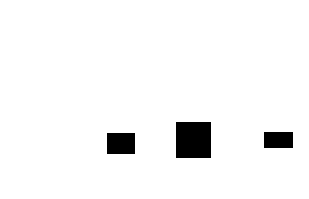
\includegraphics[width=0.4\textwidth]{afsnit/implementation/billeder/billedbehandling/binary_init}}}\hspace{1em}
    \subfloat[1. iteration]{
        \label{region1}
        \fbox{
\includegraphics[width=0.4\textwidth]{afsnit/implementation/billeder/billedbehandling/binary_s1}}}\\
    \subfloat[2. iteration]{
        \label{region2}
        \fbox{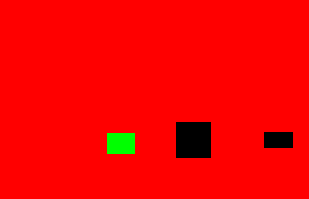
\includegraphics[width=0.4\textwidth]{afsnit/implementation/billeder/billedbehandling/binary_s2}}}\hspace{1em}
    \subfloat[3. iteration]{
        \label{region3}
        \fbox{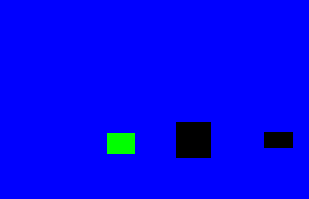
\includegraphics[width=0.4\textwidth]{afsnit/implementation/billeder/billedbehandling/binary_s3}}}\\
    \subfloat[4. iteration]{
        \label{region4}
        \fbox{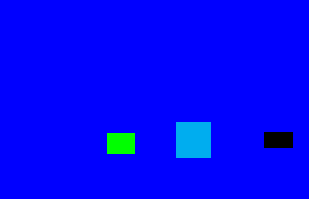
\includegraphics[width=0.4\textwidth]{afsnit/implementation/billeder/billedbehandling/binary_s4}}}\hspace{1em}
    \subfloat[5. iteration]{
        \label{region5}
        \fbox{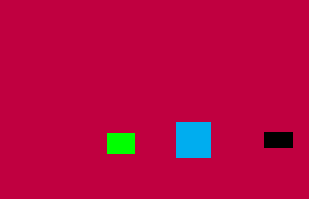
\includegraphics[width=0.4\textwidth]{afsnit/implementation/billeder/billedbehandling/binary_s5}}}\\
    \subfloat[6. iteration]{
        \label{region6}
        \fbox{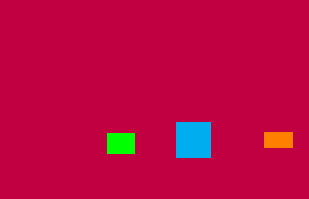
\includegraphics[width=0.4\textwidth]{afsnit/implementation/billeder/billedbehandling/binary_s6}}}\hspace{1em}
    \subfloat[7. iteration]{
        \label{region7}
        \fbox{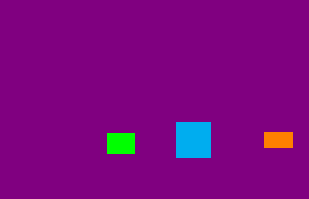
\includegraphics[width=0.4\textwidth]{afsnit/implementation/billeder/billedbehandling/binary_s7}}}
    \caption[]{Forskellige resultater med Canny kantdetektion.
    Tærskelværdierne er noteret under billederne.}
    \label{region_extract}
\end{figure}

Mere kompliceret bliver det når vi ikke har med binære billeder at gøre.
Som vist i kapitel \ref{chap_afproeving}, så vil vi, på grund af
tærskelværdierne til \texttt{cvFloodFill} og \texttt{cvCanny}, ikke
nødvendigvis finde de samme regioner med de to metoder. Vi ønsker dog at
bruge kanterne til at indikere en ny region. Derfor er det ikke nok blot
at bruge \texttt{cvFloodFill} på midten af et linjestykke mellem kanter.
Den endelige algoritme for at udtrække regioner ved et snit er den
følgende:

\vspace{0.5cm}
\begin{lstlisting}[caption={Metoder til rekonstruktion af
    kørsler},captionpos=b,label={rekonst_koersel},numbers=left]
for lineSegment in Cut:
    # Get a new color that is not in the component dictionary
    color = getRandomColor()

    for pixel in lineSegment:

        # Check if the color of the pixel equals color
        if not (color(pixel) ==  color):

            # Check if the color of the pixel are in the saved regions
            if not (color(pixel) in savedRegions):
                cv.cvFloodFill(picture, pixel, color, lowerThres, upperThres, region)

    # Color the last pixel again to make sure that the returned component is the entire region
    cv.cvFloodFill(out, pixel, color, lowerThres, upperThres, region)

    # Put the results in the component dictionary
    saveRegion(color, region)
\end{lstlisting}

Udvid til margin.

\subsection{Usikkerheder}
Hver gang vi bruger \texttt{cvFloodFill} vælges en tilfældig farve til
regionen. Her skal man være opmærksom på at man kan være uheldig og
vælge en farve som allerede bliver brugt i billedet.

``Skæve'' kanter.


%\begin{figure}[!h]
%    \centering
%    \begin{picture}(240,30)
%        \color{black}
%        \put(0, 10){$A$}
%        \put(233, 10){$B$}
%
%        \linethickness{5mm}
%        \put(85, 0){\line(1, 0){20}}
%
%        \linethickness{9mm}
%        \put(137, 3){\line(1, 0){24}}
%
%        \linethickness{3mm}
%        \put(203, 3){\line(1, 0){21}}
%
%        \linethickness{0.2mm}
%        \put(3, -5){\line(0, 1){10}}
%
%        \put(236, -5){\line(0, 1){10}}
%
%        \put(3, 0){\line(1, 0){233}}
%    \end{picture}
%    \caption[]{Eksempel på regioner der krydser snittet.}
%    \label{impUdtraek_regioner_snit}
%\end{figure}

}

% vim: set tw=72 spell spelllang=da:
